\section{Generalization Error} \label{sec:svm:generalization}
\lecture[12]{2024-02-27}{Linear SVM classifiers for linearly non-separable data:
VC Dimension}

\begin{theorem}[FOML 5.4] \label{thm:svm:error}
    Let $h_\mcD^{SVM}$ be the classifier returned by the SVM for a sample
    \mcD{}, and let $N_{SV}(\mcD)$ be the number of support vectors that
    define $h_\mcD^{SVM}$.
    Then, \[
        \E_{\mcD \sim P^m}(R(h_\mcD^{SVM}))
            \le \E_{\mcD \sim P^{m+1}}\left[\frac{N_{SV}(\mcD)}{m+1}\right]
    \]
\end{theorem}
\begin{proof}
    The proof is identical to that of \cref{thm:perceptron:error},
    proceeding via the leave-one-out error.
\end{proof}

If the training set error is zero, is the generalization error also zero?
\begin{fact}
    Let $Z_1, \dots, Z_n$ be iid random variables with
    $\Pr(Z_i \in [a, b]) = 1$ and $\E[Z_i] = \mu$.
    Then, \[
        \Pr\paren{\abs{\wbar{Z} - \mu} \ge \epsilon}
            \le 2\exp\paren{\frac{-2n\epsilon^2}{(b-a)^2}}
    \] where $\wbar{Z} = \frac{1}{n}\sum_{i=1}^n Z_i$.
\end{fact}
We can use this to give probabilistic bounds on the generalization error
using its expected value (since it is bounded between 0 and 1).

\section{VC Dimension} \label{sec:svm:vc}
Let $\mcH$ be a hypothesis class.
That is, a set of functions from $\mcX$ to $\mcY$.
For our purposes, $\mcY = \pms$.

\begin{definition}[Growth function] \label{def:vc:growth_function}
    The growth function $\Pi_\mcH\colon \N \to \N$ is defined by \[
        \Pi_\mcH(m) = \max_{x_1, \dots, x_m \in \mcX}
            \#\set{(h(x_1), \dots, h(x_m)) \mid h \in \mcH}
    \]
\end{definition}
In other words, $\Pi_\mcH(m)$ is the maximum number of distinct ways
in which $m$ points can be classified by functions in $\mcH$.
\begin{notation}
    We will denote the set of affine classifiers from $\R^d$ to $\pms$
    by $\mcL_d$.
\end{notation}
\begin{example}
    If $\mcH = \mcL_2$, then \begin{align*}
        \Pi_\mcH(1) &= 2 \\
        \Pi_\mcH(2) &= 4 \\
        \Pi_\mcH(3) &= 8
    \end{align*}
    \begin{center}
        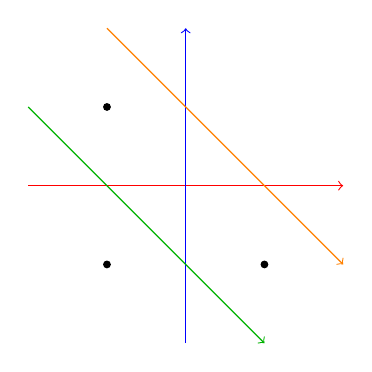
\begin{tikzpicture}
            \draw (0, 0) node[circle, fill, inner sep=1pt] (a) {};
            \draw (2, 0) node[circle, fill, inner sep=1pt] (b) {};
            \draw (0, 2) node[circle, fill, inner sep=1pt] (c) {};
            \draw[->, Red] (-1, 1) -- (3, 1);
            \draw[->, blue] (1, -1) -- (1, 3);
            \draw[->, green!70!black] (-1, 2) -- (2, -1);
            \draw[->, orange] (0, 3) -- (3, 0);
        \end{tikzpicture}
    \end{center}
    These four classifiers give four distinct ways to classify the given
    three points.
    Reversing these gives another four ways.
    There are only eight possible labelings, so $\Pi_\mcH(3) = 8$.
\end{example}

However, $\Pi_\mcH(4) < 16$.
That is, no matter which $4$ points we choose, we can't find $16$ distinct
classifications of them by functions in $\mcH$.
In other words, for any $4$ points, there exists a labeling of them
that cannot be achieved by any function in $\mcH$.

\begin{theorem*} \label{thm:vc:2}
    $\Pi_{\mcL_2}(4) < 16$.
\end{theorem*}
\begin{proof}
    Let $P$, $Q$, $R$ and $S$ be any four points, colored red or blue.
    The key observation is that if a line $L$ separates the red points
    from the blue points, then for any two points $A$ and $B$,
    $L$ intersects the line segment $\wbar{AB}$ iff $A$ and $B$ are
    colored differently.

    If any three points $P$, $Q$ and $R$ are collinear in that order,
    color them red, blue and red respectively.
    Then any line separating the red points from the blue points must pass
    through both $\wbar{PQ}$ and $\wbar{QR}$.
    The only line that does this is the line $\wbar{PR}$ itself, which
    will assign the same color to each of these.

    Now suppose that $P$, $Q$, $R$ and $S$ are such that no three are
    collinear.
    If they form a convex quadrilateral,
    color them alternately red and blue.
    \begin{center}
        \begin{tikzpicture}[every node/.style={circle, fill, inner sep=1pt}]
            \draw (0, 0) node[color=Red, label=below left:{$P$}] (P) {};
            \draw (2, 0) node[color=blue, label=below right:{$Q$}] (Q) {};
            \draw (3, 1.5) node[color=Red, label=above right:{$R$}] (R) {};
            \draw (0.5, 3.5) node[color=blue, label=above left:{$S$}] (S) {};
            \draw (P) -- (Q) -- (R) -- (S) -- (P);
        \end{tikzpicture}
    \end{center}
    Any line separating the red points from the blue points must intersect
    every side of the quadrilateral, which is not possible.

    If they form a non-convex quadrilateral, the convex hull must be a
    triangle.
    Color the points of the triangle red, and the interior point blue.
    \begin{center}
        \begin{tikzpicture}[every node/.style={circle, fill, inner sep=1pt}]
            \draw (0, 0) node[color=Red, label=below left:{$P$}] (P) {};
            \draw (1.2, 1.7) node[color=blue, label=below right:{$Q$}] (Q) {};
            \draw (3, 1.5) node[color=Red, label=above right:{$R$}] (R) {};
            \draw (0.5, 3.5) node[color=Red, label=above left:{$S$}] (S) {};
            \draw (P) -- (R) -- (S) -- (P);
        \end{tikzpicture}
    \end{center}
    A separating plane can pass through none of the sides of the triangle,
    so it cannot enter the interior of the triangle at all, and thus
    cannot separate $Q$ from the other points.
\end{proof}

\begin{definition}[Shattering] \label{def:svm:vc:shattering}
    A hypothesis class $\mcH \subseteq \mcY^\mcX$ is said to \emph{shatter}
    a set $C \subseteq \mcX$ if for every labelling of $C$ by $\mcY$,
    there exists a function $h \in \mcH$ that achieves that labelling.
    That is, \[
        \forall y \in \mcY^C \;\exists h \in \mcH
            \;\forall x \in C (h(x) = y(x))
    \]
\end{definition}
\begin{example}
    From the above theorem, we conclude that $\mcL_2$ shatters no set of
    four points.

    From the example preceding it, we conclude that the set of linear
    classifiers in $\R^2$ shatters that particular set of three points
    (and indeed, any set of three points that are not collinear).
\end{example}

\begin{definition*}[VC-dimension] \label{def:svm:vc}
    The \emph{VC-dimension} of a hypothesis class $\mcH \subseteq \mcY^\mcX$
    is the size of the largest set that can be shattered by $\mcH$.
    That is, \[
        \VC(\mcH) = \max\set{m \mid \Pi_\mcH(m) = \abs{\mcY}^m}
    \]
\end{definition*}
\begin{example}
    The VC-dimension of the set of linear classifiers in $\R^2$ is $3$.
    This is because it shatters at least one set of three points,
    but no set of four points.
\end{example}

\begin{theorem*} \label{thm:vc:linear}
    The VC-dimension of the set of linear classifiers from $\R^d$ to $\pms$
    is $d+1$.
\end{theorem*}
\begin{proof}
    Induction.
    For $d = 1$, the points $-1$ and $1$ can obviously be shattered,
    using the affine maps $x \mapsto x$, $x \mapsto -x$, $x \mapsto x + 2$
    and $x \mapsto -x - 2$.

    Also, any three points are collinear, so they cannot be shattered by
    the same argument as in the proof of \cref{thm:vc:2}.
    Thus $\VC(\mcL_1) = 2$.

    Suppose that $\VC(\mcL_{d-1}) = d$.
    Then let $P_1, \dots, P_d$ be a set shattered by $\mcL_{d-1}$.
    Let $Q_i = (P_i, 0)$ for $i = 1, \dots, d$,
    and $Q_{d+1} = (0, \dots, 0, 1)$.
    We claim that the set $\set{Q_1, \dots, Q_{d+1}}$ can be shattered
    by $\mcL_d$.

    Fix a coloring $y$ of $\set{Q_1, \dots, Q_{d+1}}$.
    Consider the same coloring applied to $\set{P_1, \dots, P_d}$
    (each $P_i$ colored the same as $Q_i$).
    Let $h(x) = \sgn(\innerp w x + b)$ be the classifier that achieves this
    coloring.
    WLOG assume that $Q_{d+1}$ is colored $+1$.
    Let $w' = (w, 1-b)$.
    Then $h(x) = \sgn(\innerp{w'}{x} + b)$ achieves the coloring $y$ of
    $\set{Q_1, \dots, Q_{d+1}}$.
    Thus $\VC(\mcL_d) \ge d+1$.

    To show that $\VC(\mcL_d) < d+2$, consider any set of $d+2$ points
    in $\R^d$.
    Suppose that they are shattered by $\mcL_d$.
    Fix a coloring $y$ of these points.
    Consider the same coloring applied to any $d+1$ points, viewed as
    points in $\R^{d-1}$.
    Since there exists a classifier that achieves this coloring in
    $\R^d$, its restriction to $\R^{d-1}$ achieves the same coloring
    in $\R^{d-1}$.
    But this is impossible, since $\VC(\mcL_{d-1}) = d$.
    Thus $\VC(\mcL_d) < d+2$.

    Winduction.
\end{proof}

\begin{fact*} \label{thm:vc:restricted_linear}
    Let \begin{align*}
        \mcX &= \set{x \in \R^d \mid \norm{x} \le R}, \text{ and} \\
        \mcH_B &= \set{h \in \pms^\mcX \mid h = \sgn(\innerp w \cdot + b)
            \text{ for some } \norm{w} \le B}
    \end{align*}
    be a class of linear classifiers on the ball $\mcX$.
    Then \[
        \VC(\mcH_B) \le B^2 R^2
    \]
\end{fact*}

Why are we interested in the VC-dimension at all?
\begin{fact*} \label{thm:vc:bound}
    Let $\mcH$ be a family of functions taking values in $\pms$
    with VC-dimension $V$.
    Then, for any $\delta > 0$, with probability at least $1-\delta$,
    the following holds for all $h \in \mcH$. \[
        R(h) \le R_{\text{emp}}(h)
            + \sqrt{\frac{V}{N} (\log N - \log \delta)}.
    \]
    \textcolor{exercise}{What the fuck does this mean?}
\end{fact*}

\begin{corollary}
    For any $h \in \mcH_B$ defined in \cref{thm:vc:restricted_linear},
    with probability at least $1-\delta$, \[
        R(h) \le R_{\text{emp}}(h)
            + O\paren{\frac{RB}{\sqrt N}}
    \]
    \textcolor{exercise}{Where did the $\log N$ go?}
\end{corollary}

This motivates the following formulation of the SVM problem for
linearly non-separable data, since smaller $w$ gives smaller bounds on
the error.
\[
    \min_{w, b} \frac12 \norm{w}^2
        + C \sum_{i=1}^{n} \paren{1 - y_i (\innerp{w}{x^{(i)}} + b)}_+
\] where $(x)_+ = x [x \ge 0] = 0 \vee x = \max(0, x)$,
and $C$ is a penalty for wrong answers.
